\chapter{The GPT Family}

Evalution of GPT models:

\begin{itemize}
  \item GPT-1 (2018): First in a (long series) of models. Decoder-only transformer architecture. Pretraining on a large corpus, fine-tuning on various tasks
  \item GPT-2 (2019): Larger training set. Initial controversies around the (lack of) release for potential misuse
  \item GPT-3 (2020): Scaling up: 175B parameters & more data!
  \item GPT-4 (2023): OpenAI no longer providing information on the model.
\end{itemize}

\section{GPT-1 (Generative Pre-trainined Transformer)}

\begin{center}
  \begin{minipage}{0.65\linewidth}
    Decoder-only transformer, pretrained on the text
    generation task.
    Training done with:
    \begin{itemize}
      \item \textbf{Unsupervised pretraining}:  next tocken prediction, can be done on large datasets
      \item \textbf{Supervised fine-tuning}: on supervides datasets such as sentiment analysis. Typically done
            on smaller datasets, this is more expensive.
    \end{itemize}
  \end{minipage}%
  \hfill
  \begin{minipage}{0.3\linewidth}
    \centering
    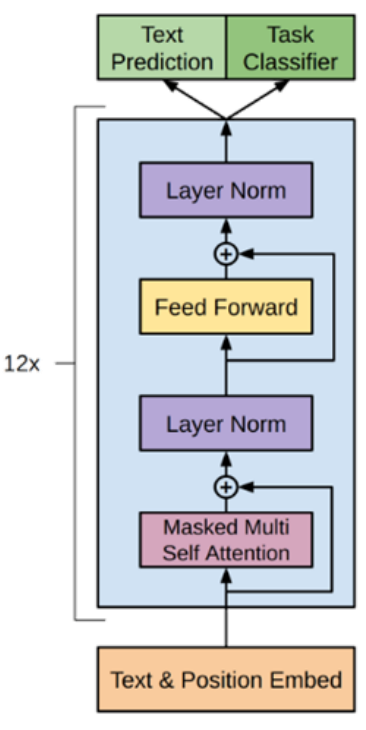
\includegraphics[width=0.3\linewidth]{content/Parts/images/2026-10-12-10-11-27.png}
  \end{minipage}
\end{center}

\subsection{GPT-1 Architecture \& tasks}

\begin{figure}[h!]
  \centering
  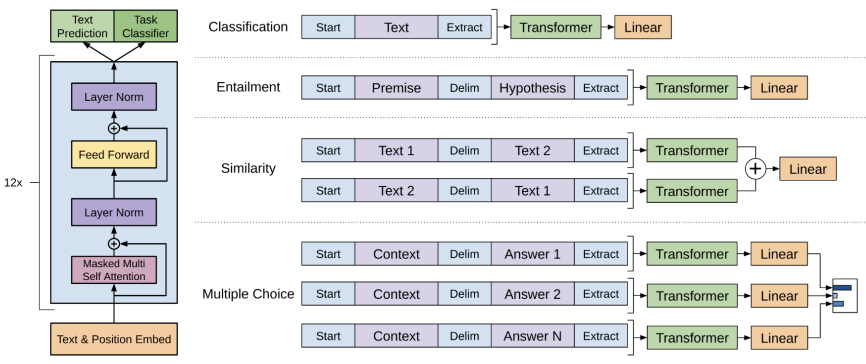
\includegraphics[width=0.3\linewidth]{content/Parts/images/2026-10-12-10-14-17.png}
\end{figure}


\subsection{GPT-1 setup}

It was unsupervised pre-trained on the BooksCorpus dataset (800M words), 7K books of
various genres. Approximately 5GB of text.

The fine-tuning was done using:

\begin{itemize}
  \item Natural languafe inference
  \item Question answering
  \item Semantic similarity
  \item Text classification
\end{itemize}

The architecture of this model is:

\begin{itemize}
  \item 12 layers decoder-only with 12 heads each
  \item 768 dimensdimensional state
  \item BPE with 40K merges
  \item Leared positional embeddings
  \item Context window of 512 tokens (WHAT!!?)
  \item 117M parameters
\end{itemize}

\section{GPT-2}

Realised in 2019, based on GPT-1 recipe, with lager training corpus (10x) and large model (10x).
It was trained with unsupervised pretraining with no \textbf{fine-tuning}.

GPT-2 shows emergent capabilities. It could solve problems it was not explicitly trained on!

"Increasing [model capacity] improves performance in a log-linear fashion
across tasks"

"Due to concerns about large language models being used to generate
deceptive, biased, or abusive language at scale, we are only releasing
a much smaller version of GPT-2 along with sampling code"

\subsection{GPT-2 setup}

Only unsupervised pretraining. Now they used WebText dataset (more data but less quality).
Text from 45M links (40GB of text), semi-curated results - links from Reddit posts with
at least 3 upvotes.


Fine-tuning is no longer used.


\subsection{Architecture}

\begin{itemize}
  \item Same as GTP-1
  \item BPE with 50257 tokens
  \item Context window of 1024 tokens
  \item Up to 1.5B parameters
\end{itemize}

\section{Scaling Laws for Neural Language Models}

Published in January 2020, by OpenAI. Shows various empirical takeaways.
There are some scaling laws and the parameters are:

\begin{itemize}
  \item Model size (number of parameters)
  \item Dataset size (number of tokens)
  \item Compute budget (number of FLOPs)
\end{itemize}

This is not a so obvious result, of cource it can be expected, but with that paper they show
the formula that can be used to predict the performance of a model.


\begin{figure}[h!]
  \centering
  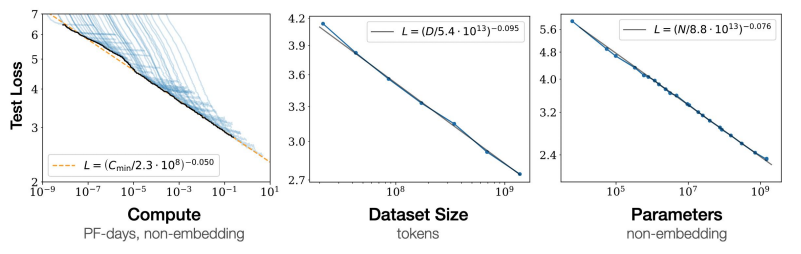
\includegraphics[width=0.3\linewidth]{content/Parts/images/2026-10-12-10-30-21.png}
\end{figure}

The Test Loss tell us how a model is performing on unseen data.


\paragraph{Other takeaways}

The model size is what is matter in that years. They see that fixing the number of parameters
of a model and scaling the transformer depth, width are not as effective as scaling the model size.

The second thing is there is a law:

\begin{equation*}
  N \propto C^{0.73}, B \propto C^{0.24}, S \propto C^{0.03}
\end{equation*}

Where N = model size, B = batch size, S = number of steps, C = computing
budget.

"As the computational budget C increases, it should be spent primarily on
larger models, without dramatic increases in training time or dataset size".

10x more computing budget $\rightarrow$ 5.4x model size, 1.7x batch size, 1.07x training
steps


\section{GPT-3}

\begin{center}
  \begin{minipage}{0.65\linewidth}

    Jennuray in 2020 published the paper we have already discussed, than in june 2020 OpenAI
    released GPT-3.
    It has 175B parameters, 10x more than GPT-2 with no other meaningful changes.

    It was trained on CommonCrawl, after filtering, WebText2, Books1, Books2, Wikipedia

    It bacame a generalistic model.

  \end{minipage}%
  \hfill
  \begin{minipage}{0.3\linewidth}
    \centering
    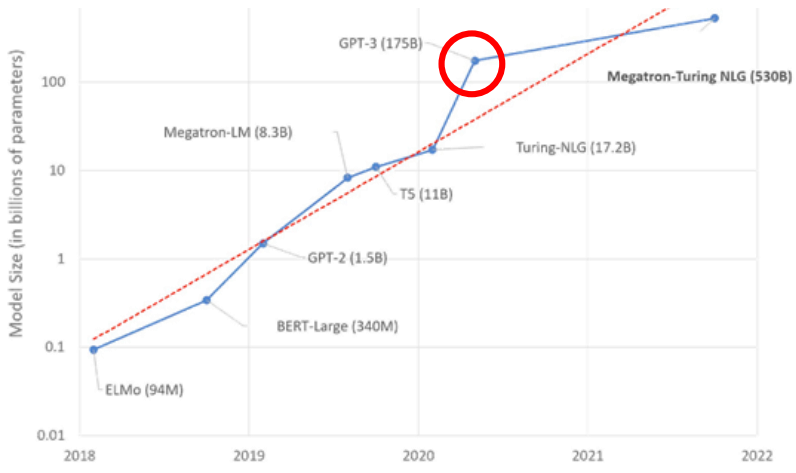
\includegraphics[width=0.3\linewidth]{content/Parts/images/2026-10-12-10-40-50.png}
  \end{minipage}
\end{center}


\section{Fine -tuning vs in -context}




\begin{center}
  \begin{minipage}{0.65\linewidth}
    How do we solve problems before GPT-3?

    \paragraph{Fine-tuning} Update model weights on a task-specific dataset.  Previously considered the
    go-to approach. No fine -tuning done on GPT -3 in -context learning only!

    \paragraph{In-context learning } this is new way to solve problems beacuse it has
    seen a lot of exampple and the solution is already into the weights.
    Model weights no longer updated. Task described as a part of the prompt in natural
    language.

    Now instaed of translating a sentence from English to French using fine-tuning,
    we pass a desccription of the task.

    \begin{itemize}
      \item \textbf{One-shot}: No other information provided to the model. It understands, simply
      \item \textbf{One-shot}: One input/output example of provided in addition to task
            description
      \item \textbf{Few-shot}: Multiple examples of input/output pairs provided. Limited by maximum context size available


    \end{itemize}
  \end{minipage}%
  \hfill
  \begin{minipage}{0.3\linewidth}
    \centering
    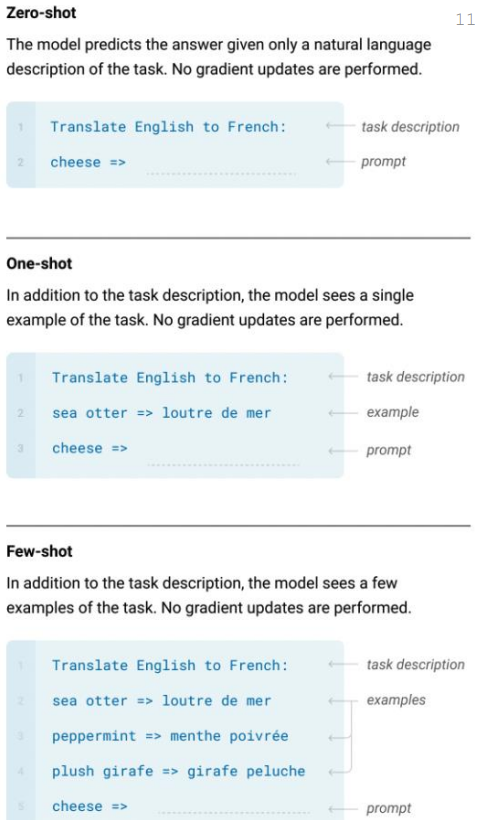
\includegraphics[width=0.3\linewidth]{content/Parts/images/2026-10-12-10-45-59.png}
  \end{minipage}
\end{center}


\subsection{In-context performance}


\begin{center}
  \begin{minipage}{0.65\linewidth}
    Larger models show remarkable 1- and few-shot performance w.r.t. smaller ones.
    The gap between 0and 1-shot performance is quite remarkable
  \end{minipage}%
  \hfill
  \begin{minipage}{0.3\linewidth}
    \centering
    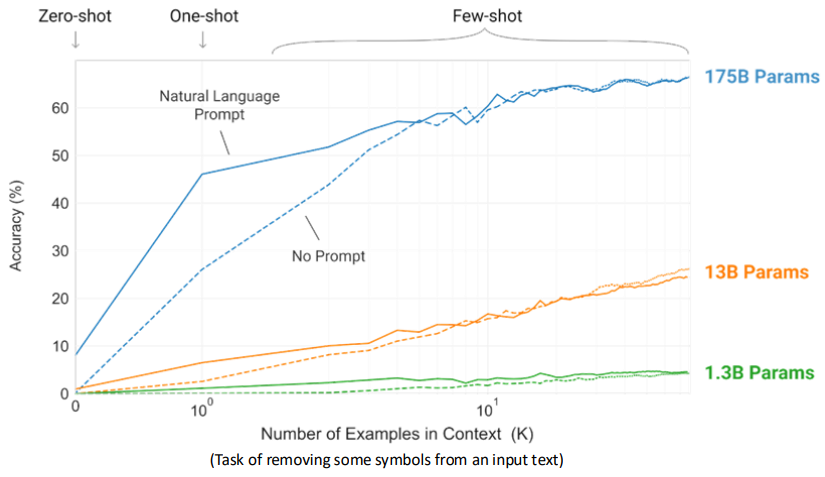
\includegraphics[width=0.3\linewidth]{content/Parts/images/2026-10-12-10-57-57.png}
  \end{minipage}
\end{center}


\subsection{Comparison with fine-tuned models}



\begin{center}
  \begin{minipage}{0.65\linewidth}
    The 175B few-shot model is comparable (or outperforms) fine-tuned SOTA models.
    In the plot: TriviaQA, but similar results on other problems.
    This is a remarkable result: Scaling the model allows not
    fine-tuning on task-specific
    datasets and still get competitive
    results!

  \end{minipage}%
  \hfill
  \begin{minipage}{0.3\linewidth}
    \centering
    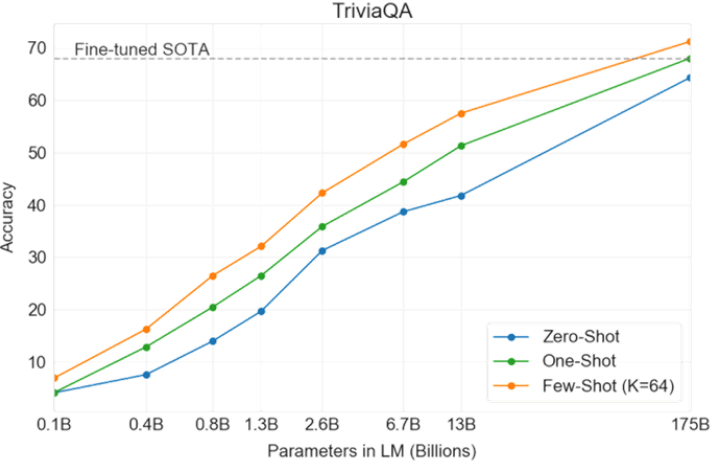
\includegraphics[width=0.3\linewidth]{content/Parts/images/2026-10-12-11-02-03.png}
  \end{minipage}
\end{center}

\subsection{The race to bigger models}


\begin{center}
  \begin{minipage}{0.65\linewidth}

    These scaling laws resulted in a
    race toward building larger
    models. GPT-3 was the first 100B+
    parameters model. Other larger models have been
    developed, following this trend
  \end{minipage}%
  \hfill
  \begin{minipage}{0.3\linewidth}
    \centering
    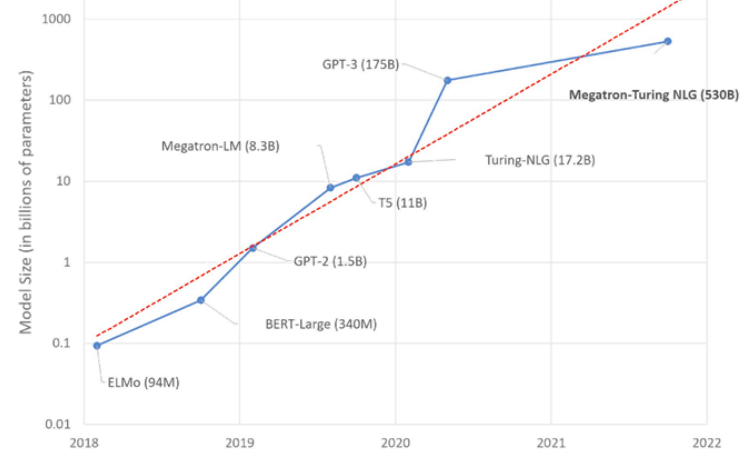
\includegraphics[width=0.3\linewidth]{content/Parts/images/2026-10-12-11-04-17.png}
  \end{minipage}
\end{center}

\section{Big models got bigger}

After the OpenAI paper lots of company has started to chase the trend of building larger models.
Reaching 500+B parameters in 2 years.

This until 2022 when DeepMind published "Training Compute-Optimal Large Language
Models".

"current large language models are significantly under-trained, a
consequence of the recent focus on scaling language models whilst keeping
  [...] data constant".


DeepMind claimed: "for every doubling of model size the number of training tokens should also be
doubled"


\subsection{Oversized and undertrained - explained}

\begin{center}
  \begin{minipage}{0.65\linewidth}

    DeepMind runs additional experiments
    with 3 approaches.

    All results indicate that the conclusions
    of Kaplan et al (2020) give too much
    importance to model size.

    For instance, the resources used for
    Gopher (280B) should have been used
    to train a 40-70B parameters model


  \end{minipage}%
  \hfill
  \begin{minipage}{0.3\linewidth}
    \centering
    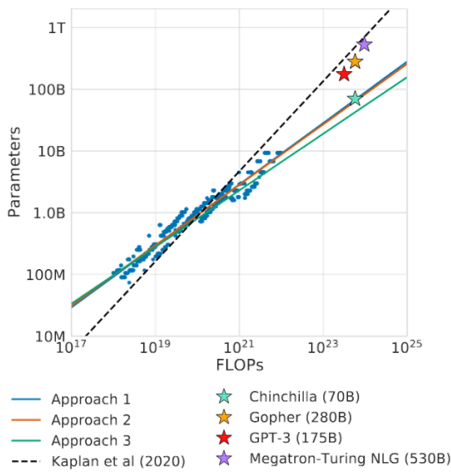
\includegraphics[width=0.3\linewidth]{content/Parts/images/2026-10-12-11-11-40.png}
  \end{minipage}
\end{center}


\section{Approach 1 (fixed-sized models)}

The first approach is empirecal, training the model.
Theu take different model with different sizes and trainig tham with different computer budget.


\section{Chinchilla}
DeepMind's presented Chinchilla, a 70B parameters model decoder-only architecture.
Trained on the same compute budget as Gopher (280B parameters).
Chinchilla is \frac{1}{4} of Gopher's size and is trained on more tokens (1.4T Chinchilla vs 0.3T Gopher).
The paper shows how Chinchilla generally outperforms Gopher, but
also GPT-3, on various tasks.

The new trend of prevous trend "always larger", is now smalled and trained for longer.


\section{Llama family}
Llama (Large Language Model Meta AI) is a family
of models introduced by Meta AI, starting in 2023.
All autoregressive, decoder-only architectures, trained on open datasets, available 
in HuggingFace.
